\section{Variability Checks}\label{app:variability}

\monika{things that are missing or we leave them out: initial conditions}

Majority of the simulations considered in this work fails to recover the \sgra observed variability in total flux.
In this Appendix we discuss and dismiss several possible causes for mismatch of $\mi{3}$ metric in models and data.

%%%%%%%%%%%%%%%%%%%%%%%%%%%%%%%%%%%%%%%%%%%%%%%%%%
%% notes from people who drafted the section

% \bp{Seems like (1) and (2) here are (or will be) discussed more thoroughly in the Numerical Methods appendix.  Given both seem to conclude that all models are consistent, and thus that changing these parameters would not reduce variability, maybe we can refer there instead of re-writing?}
%\monika{11Dec:addressed below}
%==============================================================================
% 1. GRMHD resolution.

% discussion of varying resolution [Ben to spelunk to find a 448 down set of images]

% Discussion of high resolution HAMR model.

% mapping between 230 GHz variability and accretion rate variability

%\monika{11Dec:addressed in B1}

%==============================================================================
%2. Image resolution. 

%\moinka{11Dec:addressed in B1}

%==============================================================================
%3. Model duration is not sufficiently long.

%KORAL model analysis.

%==============================================================================
%4. $\sigma_{cut}$ is overproducing variability.
% MM 11 Dec: when sigma_cut>sigma_crit  physics is unreliable and this is mentioned in the model section now. maybe not appropirate to discss here
%==============================================================================
%5. Initial conditions are not a good model.
%Comparison of Monika model initial conditions

%==============================================================================
% 6. Cooling filters the light curve. [Ben]
% \monika{11Dec:moved at the end: merged into subsection C.2}
%==============================================================================
%7. Electron distribution function model is inadequate.

%a.  Discussion of models with varying electron heating models.  Discussion of Jason's eheating models.   Forward reference to Diaz et al.  [Vedant]

%b. Discussion of models with $\Rl = 10$. [Vedant]
% \monika{11Dec:in C2}

%%%%%%%%%%%%%%%%%%%%%%%%%%%%%%%%%%%%%%%%%%%%%%%%%%

\subsection{Simulations Duration}\label{app:narayan}

\begin{figure}
  \centering
  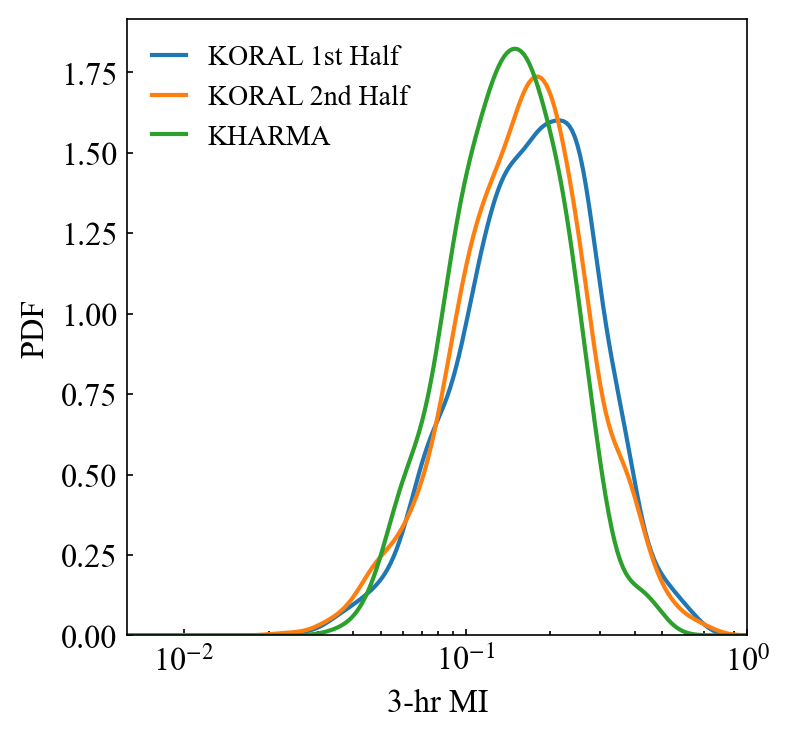
\includegraphics[width=\columnwidth]{./figures/Koral_vs_IL_MI.png}
  \caption{Distribution of \mi{3} from the full \koral model set, from the first half, from the second half, and from the comparable \kharma thermal models.}
  \label{fig:koral_MI}
\end{figure}  

Our standard models of accretion are typically evolved for $\sim 30,000 \tg$. In Figure~\ref{fig:koral_MI} we show...

insert short description of David plot with m3 for \koral vs \kharma

%==============================================================================
\subsection{Effects of $\Rl$ and radiative cooling}
\monika{i am still editing this}

For systems with sub-Eddington accretion rates, $\Dot{M}\ll\Dot{M}_{Edd}$, such as SgrA$^{*}$, radiative processes can be neglected during fluid evolution (\citealt{2012MNRAS.426.1928D, 10.1093/mnras/stw3116, Ryan_2017}) and the plasma can be considered Coulomb collisionless (\citealt{Mahadevan_1997, 10.1093/mnras/stw3116, Ryan_2017}). However, the uncertainties with electron heating and advection, and a limited understanding of the funnel warrant a discussion of cooler electrons in regions of high magnetization, and in particular, its effect on the $230GHz$ lightcurve variability. 

The $\Rh$ prescription (Equation \ref{eq:rhigh_prescription}) has three free parameters: $\Rh$, $\Rl$ and $\beta_{crit}$. During post-processing, the $\Rh$ parameter is generally varied while $\Rl$ and $\beta_{crit}$ is set to unity. In this section we investigate the effect of varying $\Rl$ on the 3 hour modulation index, $M_{3}$.

Paticle-in-cell (PIC) simulations modelling turbulent dissipation or dissipation associated with magnetic reconnection suggest preferential heating of the electrons in regions of low plasma $\beta$ (\citealt{2010MNRAS.409L.104H, Rowan_2017, 10.1093/mnras/stx2530, Rowan_2019, Kawazura771, PhysRevX.10.041050, kawazura2021energy}). The $\Rl$ parameter dictates the electron temperature in these regions, that is, in the funnel. Figure \ref{fig:rlow_comparison} shows the effect of $\Rl$ on image morphology.

\begin{figure*}
\centering
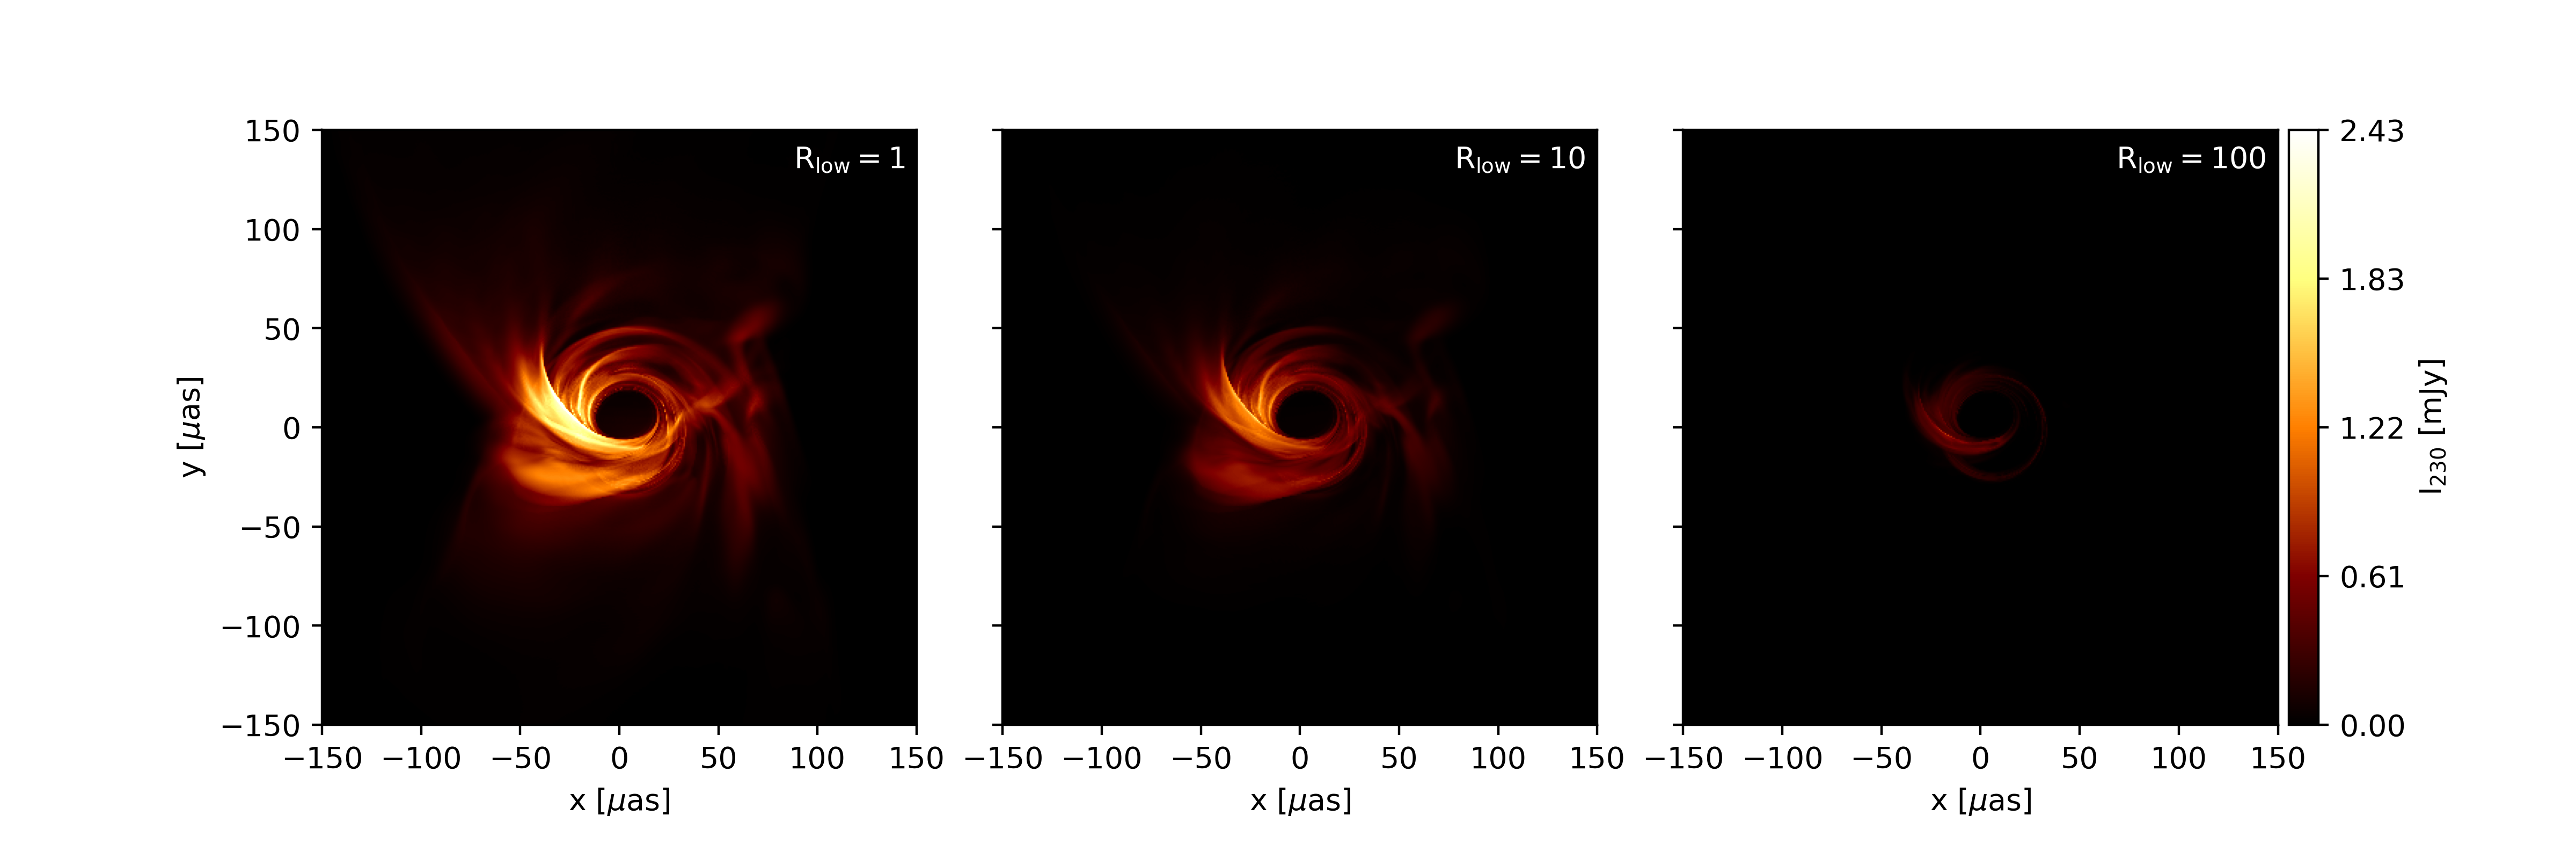
\includegraphics[width=0.95\textwidth]{figures/rlow_comparison_rhigh160.png}
\caption{Comparison of images for the same fluid snapshot with varying $\Rl$. The density scale $\mathcal{M}$, and FOV were increased to accentuate the differences between the images. The total emission in the funnel decreases with increasing $\Rl$.}
\label{fig:rlow_comparison}
\end{figure*}



We vary $\Rl$ for a select set of the best bet Illinois/Thermal models and plot the distribution of the 3 hour modulation index $M_{3}$ in Figure \ref{fig:mi_rlow}.

\begin{figure*}
\centering
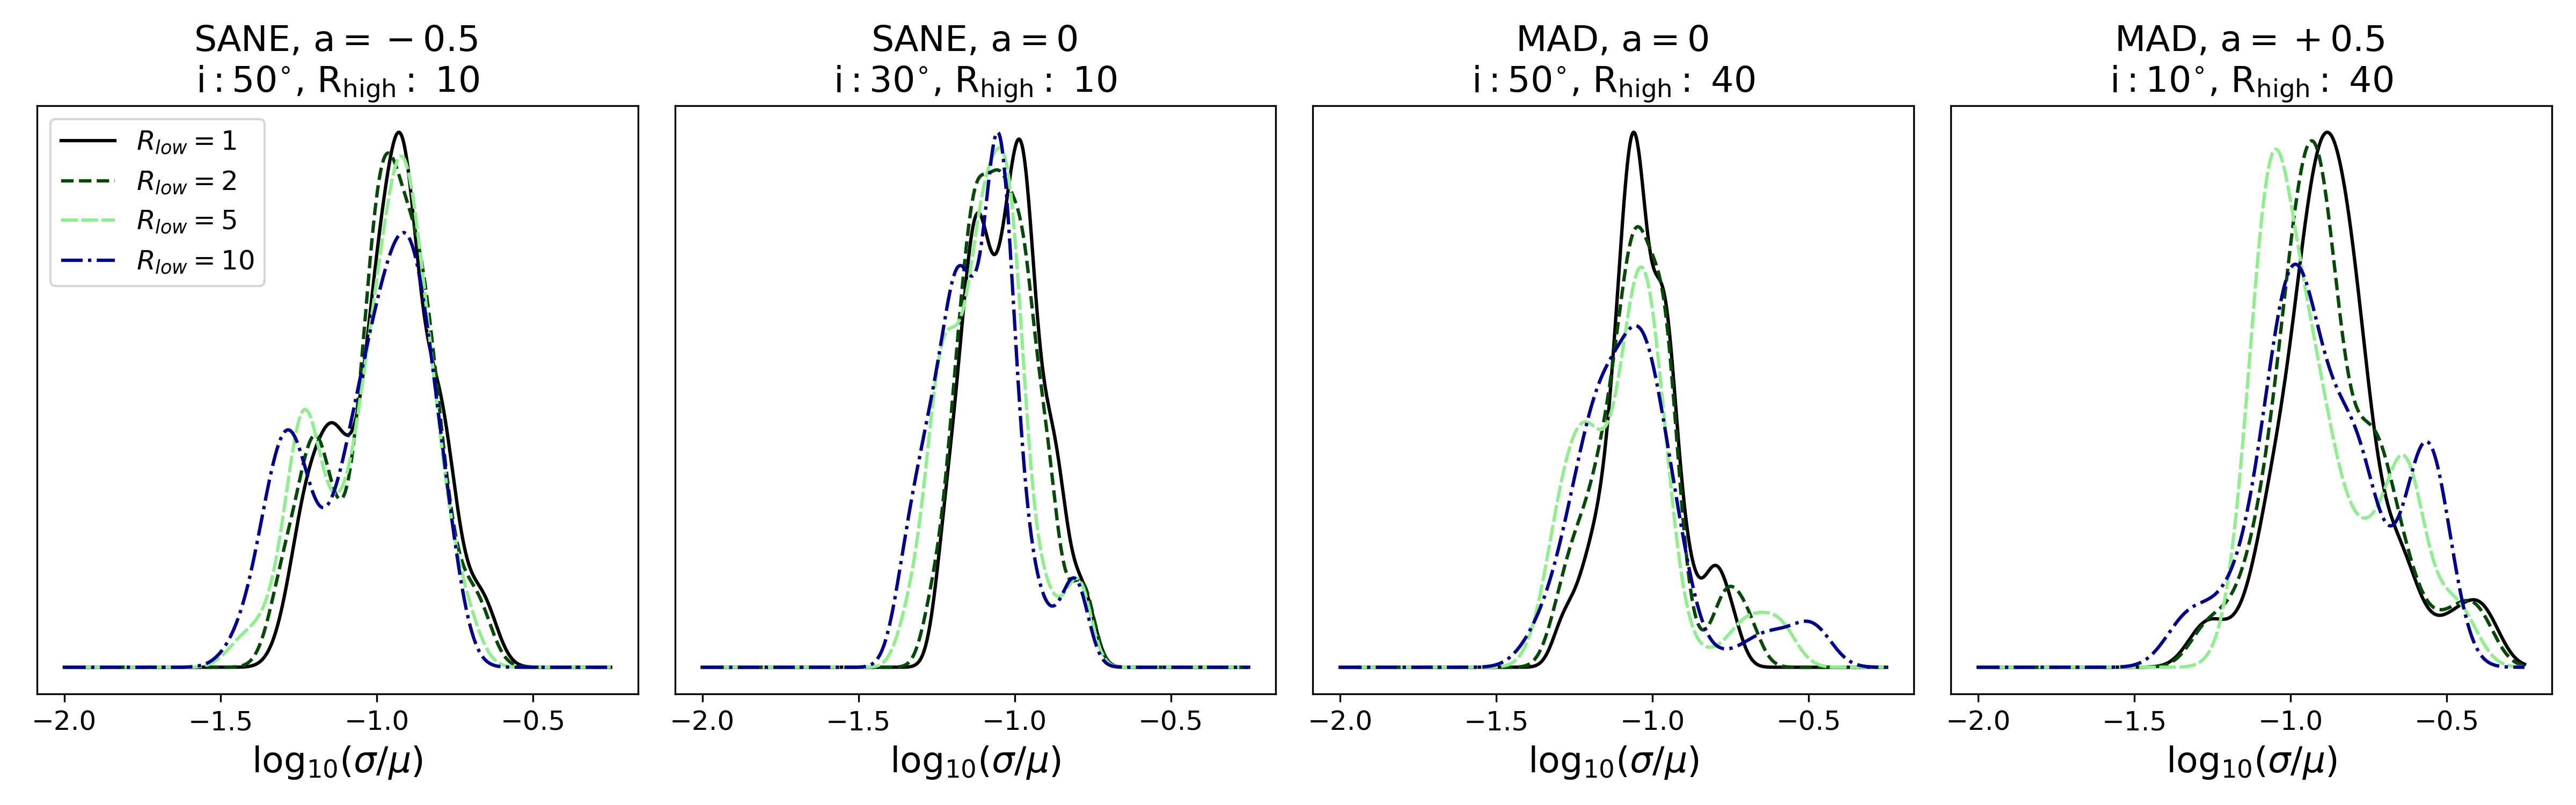
\includegraphics[width=0.95\textwidth]{figures/mi_rlow_select_models.png}
\caption{Modulation index computed over 3 hour intervals $M_{3}$, for a subset of the Illinois/Thermal models. For this analysis, we considered the (25k-30k)$GM/c^{3}$ time interval.}
\label{fig:mi_rlow}
\end{figure*}

Although the minimum value of the distribution decreases when $\Rl$ is increased, there is no clear trend for the mean of the distribution. In addition, the average $M_{3}$ still does not match observational values.


%\subsection{Radiative cooling}\label{app:cooling}

We also check if excess flux variability comes from an overestimate of electron temperatures in areas where radiative cooling of the electrons may become important. We can estimate the possible effects of this change by imposing a limit on electron temperatures based on the local dynamical time, reflecting the assumption that higher-temperature electrons would cool before crossing the event horizon.

This limit comes from comparing two timescales: the synchrotron cooling rate at high temperature,
\begin{align}
    \tau_\mathrm{cool} \approx \frac{3 m_e^3 c^5}{16 B^2 e^4 \Theta_e}
\end{align}
%dependent on the electron temperature $\Theta_e$, expressed in units of the rest mass energy, and the local field strength $B$ in Gauss. 
and the the dynamical time
\begin{align}
    \tau_\mathrm{dyn} \approx \left( r \sin{\theta} \right) ^{3/2} \frac{G M_\mathrm{BH}}{c^3}.
\end{align}

A set of images was produced which put a ceiling on the electron temperature $\Theta_e$, by requiring that the $\tau_\mathrm{cool} > N \cdot \tau_\mathrm{dyn}$ -- that is, assuming that electrons likely to cool on timescales shorter than $N$ dynamical times will do so. Lightcurves made using different values of this ceiling are shown in Figure~\ref{fig:ceiling_lc1} and the corresponding $\mi{3}$ index is shown in Figure~\ref{fig:ceiling_lc2}.

\begin{figure*}
    \centering
    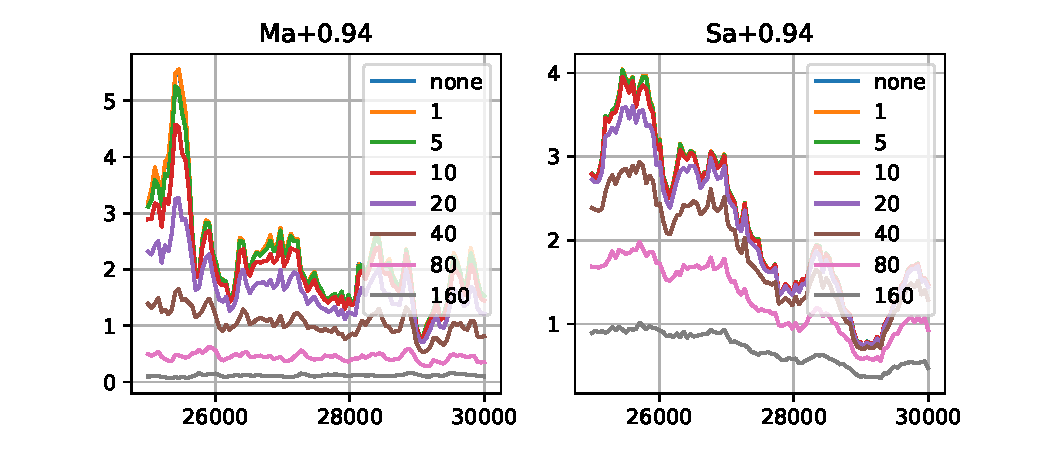
\includegraphics[width=0.95\textwidth]{figures/ctcut_lightcurves.pdf}
    \caption{Lightcurves when applying a ceiling on electron heating based on an estimate of the local electron cooling time, compared against the local dynamical time. Different values represent ceilings at different numbers of dynamical times.}
    \label{fig:ceiling_lc1}
\end{figure*}

\begin{figure*}
    \centering
    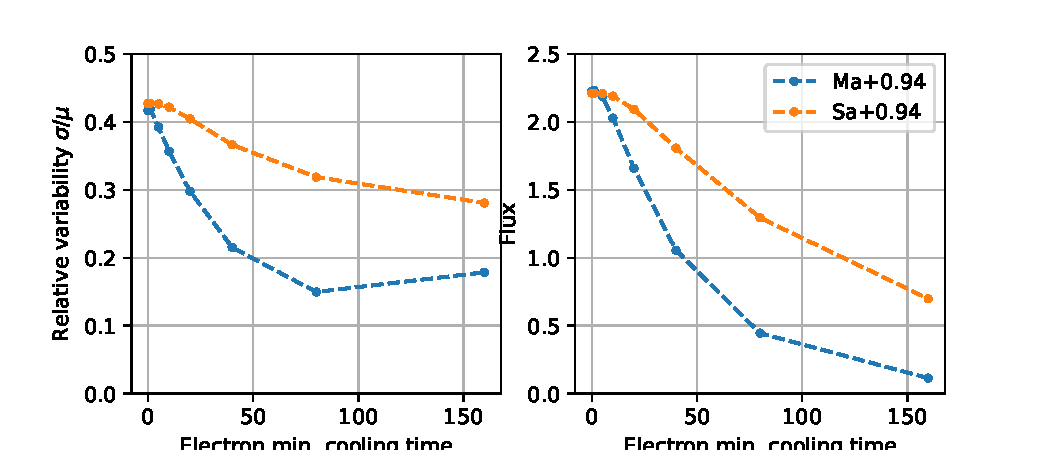
\includegraphics[width=0.95\textwidth]{figures/ctcut_effects.pdf}
    \caption{Effects of the electron temperature ceiling on lightcurve and variability in sample models.}
    \label{fig:ceiling_lc2}
\end{figure*}


%==============================================================================
%8. The flow is actually made of helium. [George]

%brief discussion, forward reference to Wong+.

% now C4



%==============================================================================
%9. $\gamma = 5/3$ rather than $4/3$.   [Vedant]  When $\gamma = 4/3$ the compression ratio across the shock is larger.

\subsection{Effects of self-consistent electron heating}

The thermal models considered in Section~\ref{sec:models} assign a local electron temperature as a post-processing step based on local magnetic field strength, parameterized by plasma $\beta$ (Equation \ref{eq:rhigh_prescription}).

\citealt{10.1093/mnras/stv2084} provided a formulation to model electron thermodynamics during the fluid evolution. Numerical dissipation at grid scale sources entropy generation and is used to heat the electrons based on a microphysical, sub-grid heating prescription. Local fluid and electromagnetic variables are used to compute the electron entropy which along with the ideal gas equation of state, can be converted into a temperature ($\Theta_{e}$). This approach allows computing the electron temperature at each timestep of the simulation, and not during post-processing, as it is done in the $\Rh$ and Critical-$\beta$ prescriptions.

We consider three sub-grid heating models that prescribe the partition of dissipated energy into electrons and ions. \citealt{2010MNRAS.409L.104H} computed the ratio of ion-to-electron heating due to dissipation of Alfv\'enic turbulent cascade, while \citealt{10.1093/mnras/stx2530} and \citealt{Rowan_2017} considered magnetic reconnection as the source of energy dissipation at sub-grid scales. These studies provide an approximate fitting formula for the ion-to-electron heating rate ($Q_{i}/Q_{e}$) based on local ion-to-electron temperature ratio ($T_{i}/T_{e}$) and local magnetic field strength -- parameterized by $\sigma$ or plasma $\beta$.

The GRMHD simulations considered here are a subset of the simulations analyzed in \citealt{2020MNRAS.494.4168D}. These include MAD and SANE accretion flows at spins, $a_{*}=0,+1/2,+15/16$. We compute the 3 hour modulation index $M_{3}$, over the time interval (5k-10k)$GM/c^{3}$. The average $M_{3}$ values are comparable to similar $\Rh$ models, with SANE reconnection models exhibiting a reduced variability as compared to the corresponding turbulent heating models. However, the average $M_{3}$ for all the models is greater than the $M_{3}$ measured from the ALMA lightcurve on three days. 

\subsection{Effects of fluid adiabatic index, $\Gamma_\mathrm{ad}$}

We expect the ions and electrons in hot accretion flows to be thermally decoupled and the resulting plasma to be two-temperature (\citealt{1976ApJ...204..187S, Quataert_1998, 10.1093/mnras/stw3116, Ryan_2018}). The electrons in such flows are relativistic and can be modelled as a fluid with an adiabatic index $\Gamma_{e}=4/3$, while the ions are nonrelativistic and possess an adiabatic index, $\Gamma_{i}=5/3$.

The adiabatic index of the fluid assumes a value between $\Gamma_{e}$ and $\Gamma_{i}$ dictated by the thermodynamics of the ions and electrons (cf. Figure 4 in \citealt{10.1093/mnras/stw3116}). Since we do not model electron thermodynamics and ignore radiative effects during our fluid simulations, we consider a constant value $\Gamma_{ad}$, and set it to 4/3 for the \textit{standard} set of simulations, ie. $\Gamma_{ad}=\Gamma_{e}$. While this may be the case in the funnel, where the electrons are the hottest and highly relativistic; the fluid adiabatic index value away from the poles can be higher than the relativistic value.

We look at the interplay between fluid adiabatic index and lightcurve variability by evaluating $M_{3}$ for thermal, GRMHD models with a higher fluid adiabatic index. This includes MAD models with $\Gamma_{ad}=13/9$ (see Section~\ref{app:narayan} and  \citealt{2021arXiv210812380N}) and SANE models with $\Gamma_{ad}=5/3$. The models exhibit lightcurve variability similar to the \textit{standard} library and have an average $M_{3}$ that is greater than the value obtained from the ALMA lightcurve. \kc{maybe discuss hamr thermal models here too}

\subsection{Effects of plasma composition}\label{app:helium}

\monika{a few sentences and short reference to forthcoming paper are missing... }

